\section{Usability Study (BYU 2019)}

\subsection*{Overview}
\begin{frame}
  \frametitle{Usability Study (BYU 2019)}

  \begin{itemize}
    \item Conducted at Brigham Young University, Utah
    \item Two independent studies:
          \begin{enumerate}
            \item Two-week study on the use of 2FA methods
                  \begin{itemize}
                    \item Login to online banking app
                    \item 12 times over course of two weeks
                  \end{itemize}
            \item Study on the setup of different 2FA methods
          \end{enumerate}
    \item Evaluation of time and usability
  \end{itemize}
  \note{
    \begin{itemize}
      \item Two parts, day-to-day usage and only setup process
      \item day-to-day
            \begin{itemize}
              \item no remember me feature
              \item every participant only one method
            \end{itemize}
      \item setup process
            \begin{itemize}
              \item every participant sets up every method
              \item can compare it
              \item tested seperately \textrightarrow maybe only setup needs to be improved or vice versa
              \item will not touch on the usability of the setup process today, since it would go beyond the scope of this presentation
            \end{itemize}
    \end{itemize}
  }

\end{frame}

\subsection{Day-to-Day Use}

\begin{frame}
  \frametitle{Time to Authenticate}

  \begin{itemize}
    \item Time from successful password entry to authentification
  \end{itemize}
  \begin{figure}[c]
    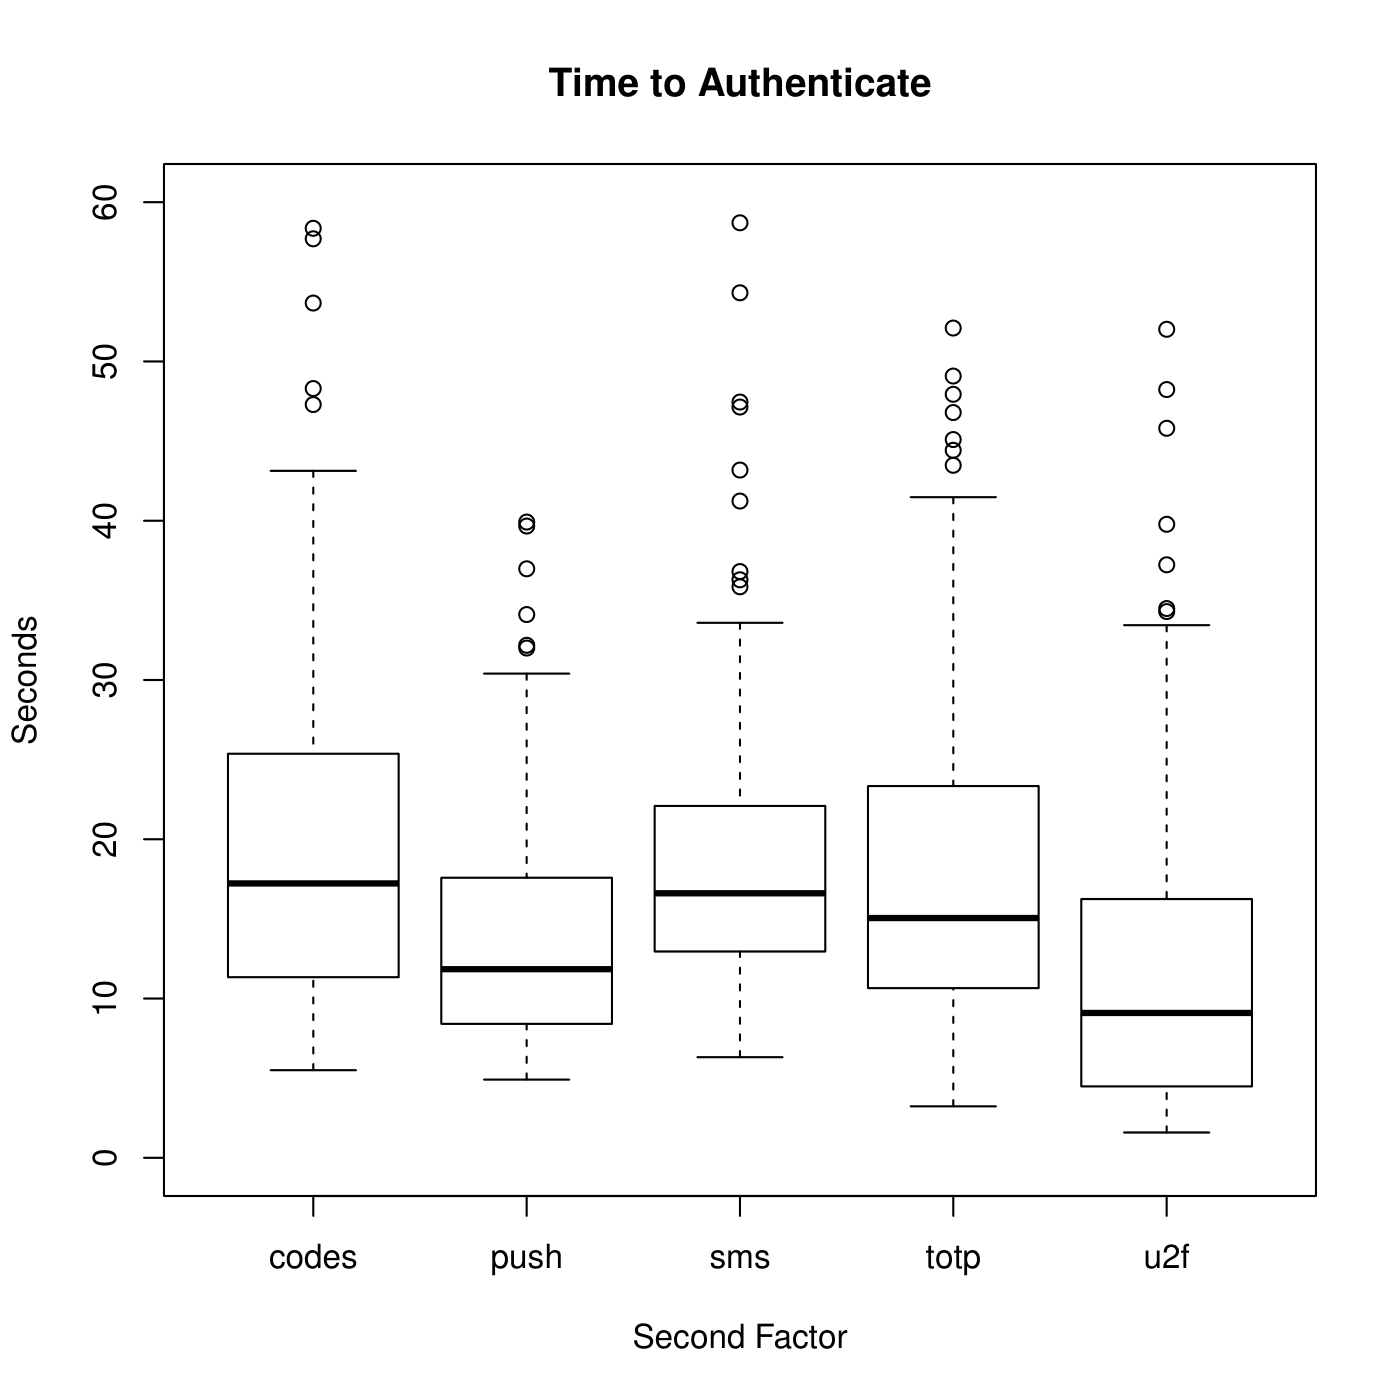
\includegraphics[height=0.8\textheight]{authentication-time}\cite{reese2019}
  \end{figure}

  \note{
    \begin{itemize}
      \item Time to enter password is not included in measured time
      \item U2F was the fastest, probably since users kept the token plugged in
      \item push notifications scored second place \textrightarrow{} prepared for authentication, phone in vincinity, good internet connection at home
      \item other three methods all require user input of confirmation code \textrightarrow{} time difference might be due to that
      \item SMS: additionaly time to send
      \item pregenerated codes might
      \item \begin{itemize}
              \item[\textrightarrow] variance quite big since different users probably store the codes differently
            \end{itemize}
    \end{itemize}
  }

\end{frame}

\begin{frame}
  \frametitle{Usability of Authentication}

  \begin{itemize}
    \item Assessment of perceived usability according to standard scale SUS\,
\includegraphics[height=0.25\baselineskip]{sus}
          {\tiny\textcolor{white}{\endnote{\url{https://borderpolar.com/wp-content/uploads/2021/06/red-among-us-png-842x1024.png.webp}}}} % chktex 29
  \end{itemize}
  \begin{figure}[c]
    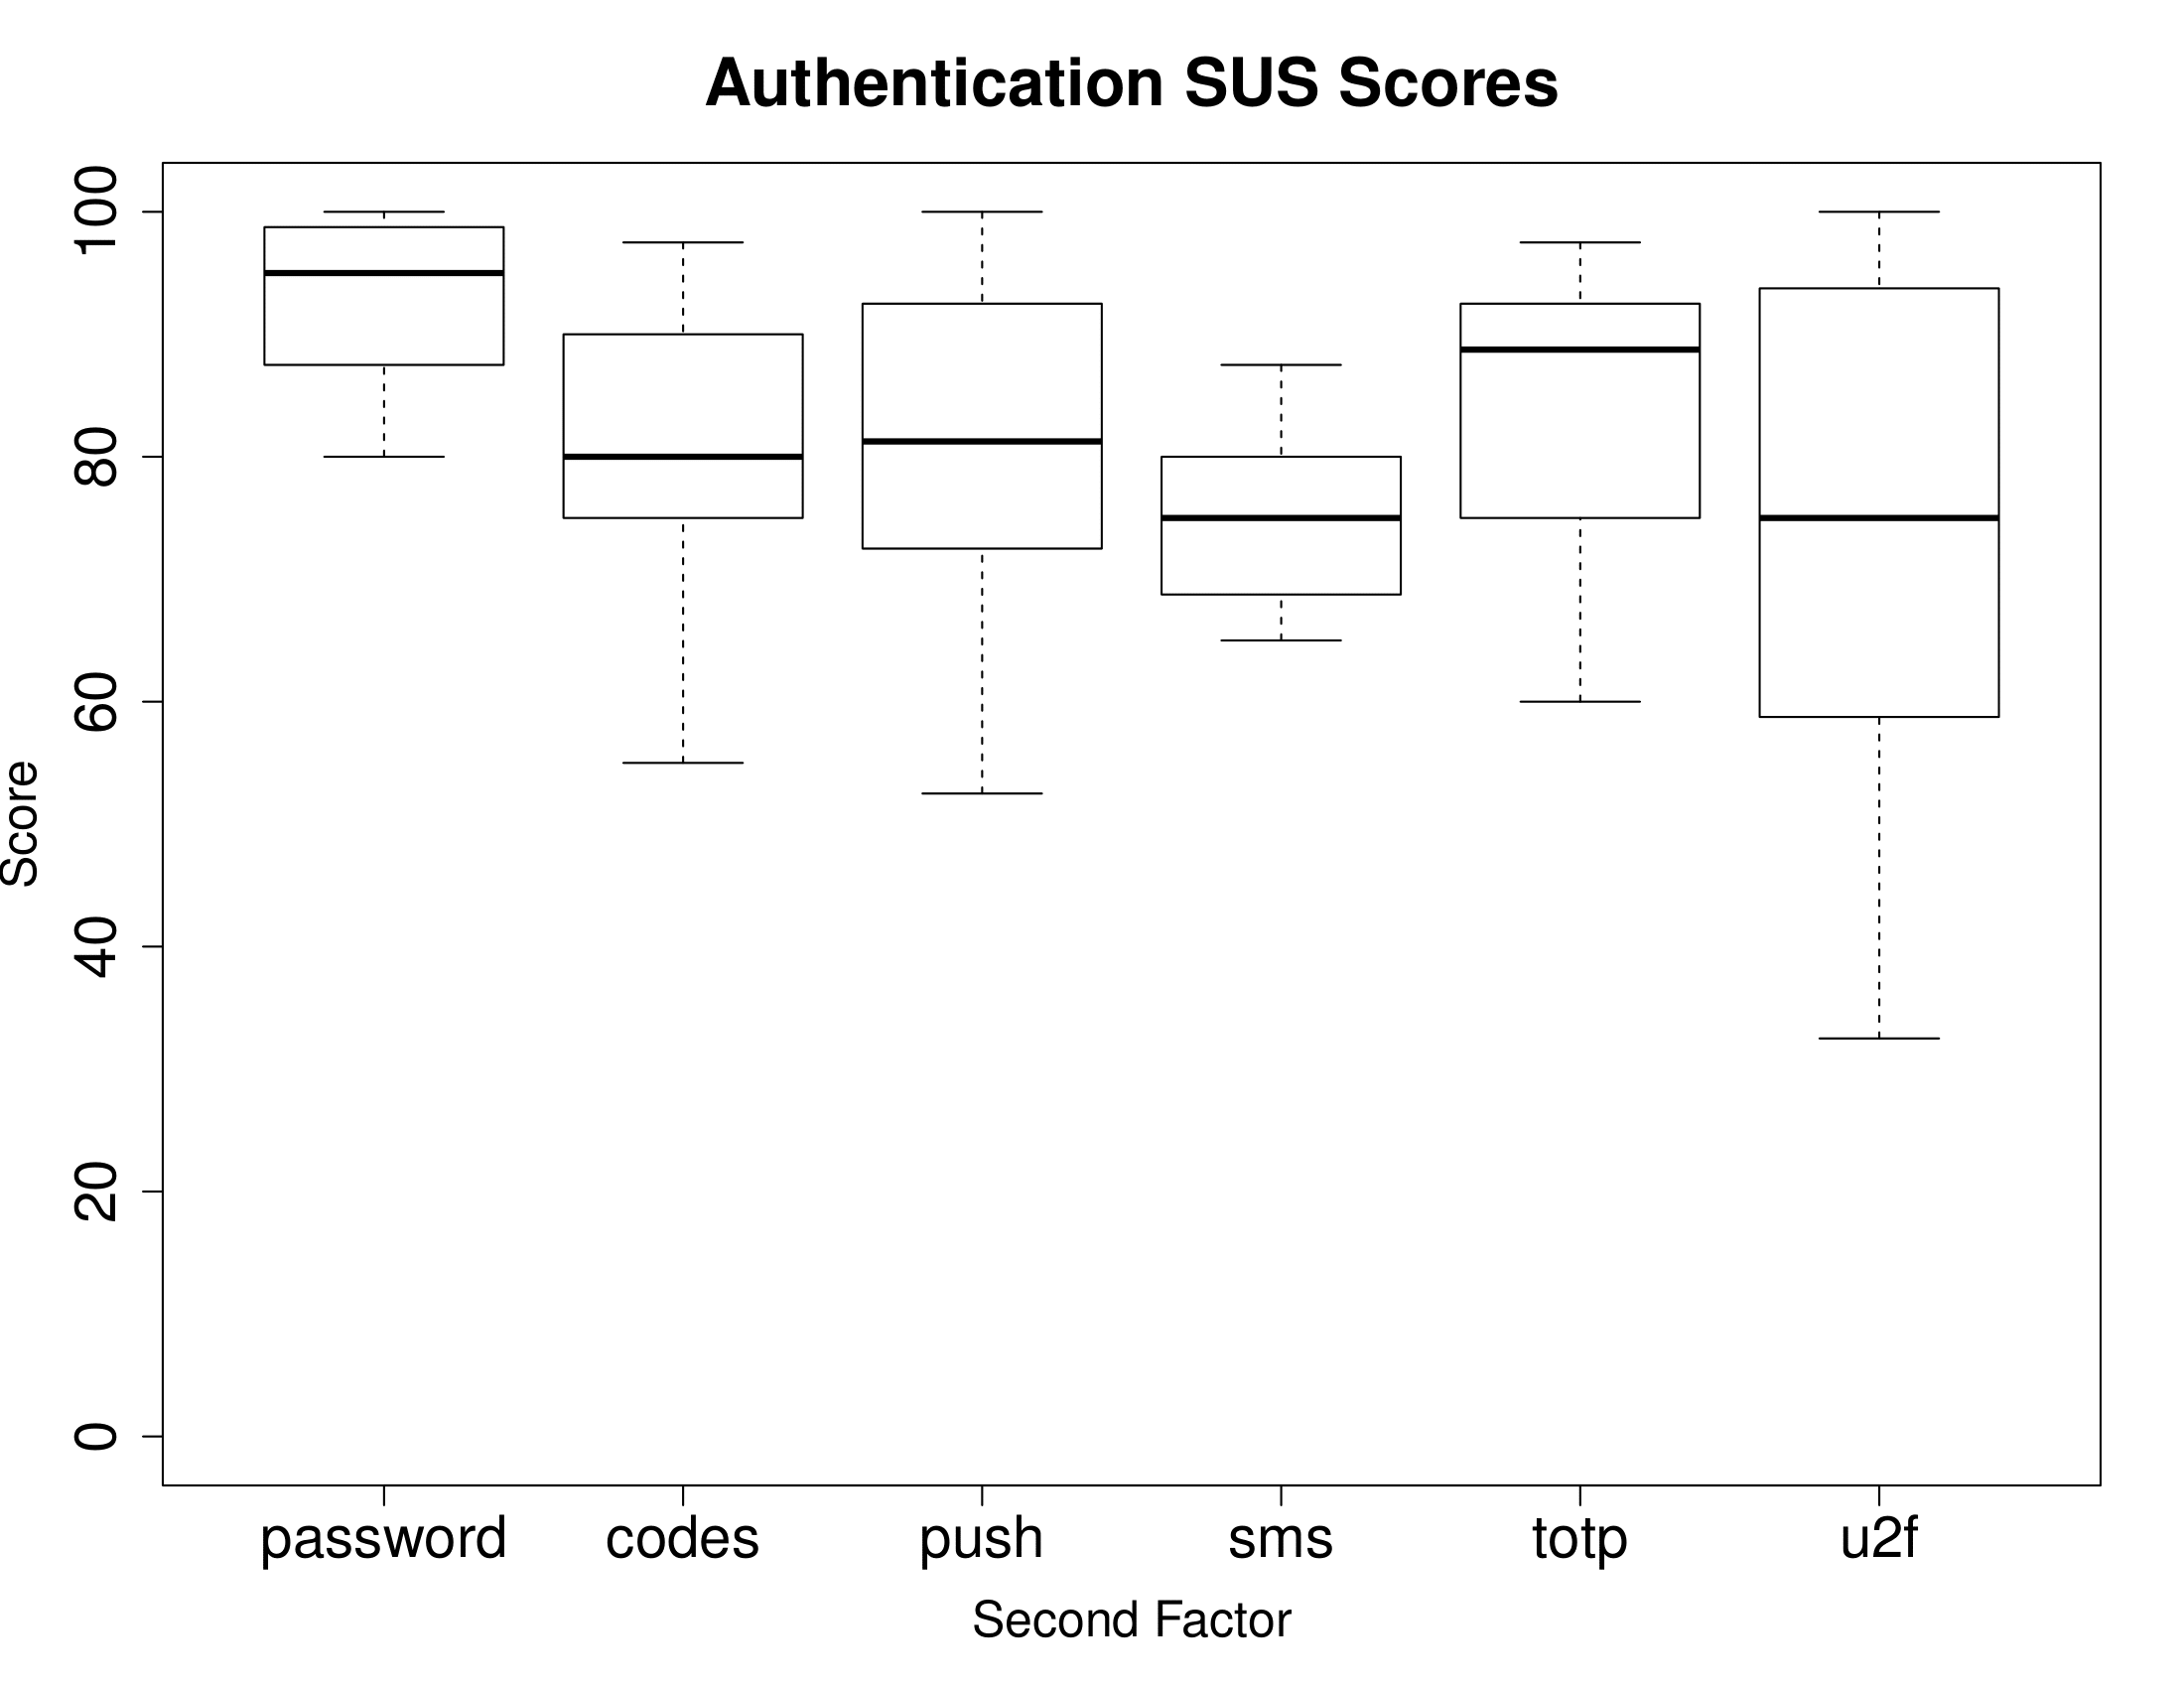
\includegraphics[height=0.76\textheight]{authentication-sus}\cite{reese2019}
  \end{figure}

  \note{
    \begin{itemize}
      \item password as control value, as you can see other values are all worse, since they only complicate the authentication
      \item while TOTP was the third slowest method, it scored best on the SUS scale
            \begin{itemize}
              \item the app that was used is probably designed very user friendly
              \item some users complained that codes would expire to quick
              \item explains longer authentication time in last slide
            \end{itemize}
      \item quite interesting to see: U2F was fastest, but has the worst usability score
            \begin{itemize}
              \item time does not seem to be the single most important factor for users
              \item differences in score, since different users might also store the security token differently
              \item[\textrightarrow] not everyone wants to have to carry another device which isn't their phone
            \end{itemize}
    \end{itemize}
  }

\end{frame}
